% !TeX document-id = {2e1841e8-ce56-4d5c-95b9-f6ac1d5fc83f}
% !TeX TXS-program:compile = txs:///pdflatex/[--shell-escape]
%\RequirePackage{fix-cm}
\documentclass[border=0pt]{standalone}
\usepackage[utf8]{inputenc}
\usepackage{lmodern}
\usepackage{graphics}
\usepackage{tikz,filecontents, pgfplots}
\pgfplotsset{compat=1.5}
\usepackage{siunitx}
\usepackage{textcomp}
\usepackage{gensymb}
\usepackage{pgfplots}
\usetikzlibrary{positioning,spy}
\usepackage{amsmath}
\usetikzlibrary{decorations,decorations.markings,decorations.text}
\usetikzlibrary{arrows,
	arrows.meta,
	decorations.pathmorphing,
	calc,%
	decorations.pathmorphing,%
	decorations.markings,
	fadings,%
	shadings,%
	positioning,
	spy,
	shapes,
	shapes.geometric,
	shapes.arrows,
	fit,
	plotmarks,}
\usetikzlibrary{arrows}

\tikzset{
	axis break gap/.initial=2mm
}

\usepackage{tikz-dimline}
\begin{document}
\begin{tikzpicture}[spy using outlines={circle,black, ultra thick,connect spies}]
\node(nsom) at (current page.center) {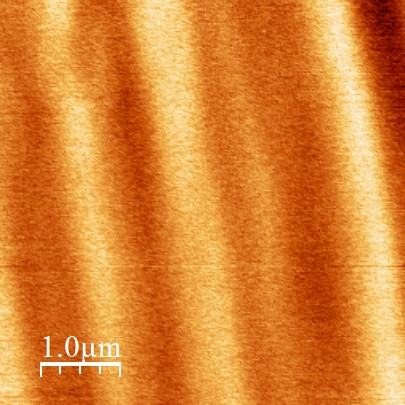
\includegraphics[scale=1]{fignsom}};

\draw[densely dashed,line width=0.8mm,white] ([xshift=-1mm,yshift=-30mm]nsom.center)--([xshift=-10mm,yshift=-40mm]nsom.north);
\draw[densely dashed,line width=0.8mm,white] ([xshift=8mm,yshift=-29mm]nsom.center)--([xshift= -1mm,yshift=-39mm]nsom.north);

\draw[line width=1mm,blue] ([xshift=-45mm,yshift=-28mm]nsom.east)--([xshift=22mm,yshift=-34mm]nsom.west);

\draw[-{stealth},line width=1.5mm,blue] ([xshift=28mm,yshift=-30mm]nsom.west)--([xshift=45mm,yshift=-27mm]nsom.west);
\end{tikzpicture}

\end{document}